\documentclass[12pt,a4]{article}
\usepackage[]{graphicx}\usepackage[]{xcolor}
% maxwidth is the original width if it is less than linewidth
% otherwise use linewidth (to make sure the graphics do not exceed the margin)
\makeatletter
\def\maxwidth{ %
  \ifdim\Gin@nat@width>\linewidth
    \linewidth
  \else
    \Gin@nat@width
  \fi
}
\makeatother

\definecolor{fgcolor}{rgb}{0.345, 0.345, 0.345}
\newcommand{\hlnum}[1]{\textcolor[rgb]{0.686,0.059,0.569}{#1}}%
\newcommand{\hlstr}[1]{\textcolor[rgb]{0.192,0.494,0.8}{#1}}%
\newcommand{\hlcom}[1]{\textcolor[rgb]{0.678,0.584,0.686}{\textit{#1}}}%
\newcommand{\hlopt}[1]{\textcolor[rgb]{0,0,0}{#1}}%
\newcommand{\hlstd}[1]{\textcolor[rgb]{0.345,0.345,0.345}{#1}}%
\newcommand{\hlkwa}[1]{\textcolor[rgb]{0.161,0.373,0.58}{\textbf{#1}}}%
\newcommand{\hlkwb}[1]{\textcolor[rgb]{0.69,0.353,0.396}{#1}}%
\newcommand{\hlkwc}[1]{\textcolor[rgb]{0.333,0.667,0.333}{#1}}%
\newcommand{\hlkwd}[1]{\textcolor[rgb]{0.737,0.353,0.396}{\textbf{#1}}}%
\let\hlipl\hlkwb

\usepackage{framed}
\makeatletter
\newenvironment{kframe}{%
 \def\at@end@of@kframe{}%
 \ifinner\ifhmode%
  \def\at@end@of@kframe{\end{minipage}}%
  \begin{minipage}{\columnwidth}%
 \fi\fi%
 \def\FrameCommand##1{\hskip\@totalleftmargin \hskip-\fboxsep
 \colorbox{shadecolor}{##1}\hskip-\fboxsep
     % There is no \\@totalrightmargin, so:
     \hskip-\linewidth \hskip-\@totalleftmargin \hskip\columnwidth}%
 \MakeFramed {\advance\hsize-\width
   \@totalleftmargin\z@ \linewidth\hsize
   \@setminipage}}%
 {\par\unskip\endMakeFramed%
 \at@end@of@kframe}
\makeatother

\definecolor{shadecolor}{rgb}{.97, .97, .97}
\definecolor{messagecolor}{rgb}{0, 0, 0}
\definecolor{warningcolor}{rgb}{1, 0, 1}
\definecolor{errorcolor}{rgb}{1, 0, 0}
\newenvironment{knitrout}{}{} % an empty environment to be redefined in TeX

\usepackage{alltt}
\newcommand{\SweaveOpts}[1]{}  % do not interfere with LaTeX
\newcommand{\SweaveInput}[1]{} % because they are not real TeX commands
\newcommand{\Sexpr}[1]{}       % will only be parsed by R



% ---- Metadata ---- %

\title{Honesty by Convenience: Corruption Tolerance in Ecuador}
\author{Daniel Hernán Sánchez Pazmiño}
\date{June 2022}

% ---- Load Packages ---- %

% Math

\usepackage{savesym} % Need to "save" the command that is already defined \varTheta

\usepackage{amsmath}
  \savesymbol{varTheta}

% Fonts

% To set the TNR font for both text and equations:

\usepackage{mathspec}
  \setallmainfonts(Digits,Greek,Latin){Times New Roman}
\restoresymbol{MTP}{varTheta}

% Formatting

\usepackage{setspace}
  \doublespacing

\usepackage[margin = 1in]{geometry}

\usepackage{lscape}

% Citation & Bibliographies

\usepackage[backend = biber, style = apa, citestyle = apa]{biblatex}
  \addbibresource{refs.bib}
  
% For tables:

 % For the modelsummary tables:
\usepackage{siunitx}
\usepackage{booktabs} 
  \newcolumntype{d}{S[input-symbols = ()]}

\usepackage{caption}
\usepackage{multirow}
\usepackage[flushleft]{threeparttable}
  
% Other packages

\usepackage{csquotes} % For quotation marks

\usepackage{epigraph} % For epigraph
  \setlength\epigraphwidth{9cm}
  \setlength\epigraphrule{1pt}

\usepackage{float} % For the H float option- only used in emergencies (lol)

\usepackage{textcomp} % For the registered trademark symbol.

% Always load these packages at the end of the preamble:

\usepackage{hyperref}

% ---- R Stuff to be used in the whole document ----

% Here I will execute or source R code through chunks that I need to use throughout the whole document.

% General settings



% Load the data by sourcing the data manipulation script. Note that survey design objects are indeed created in this script.




\begin{document}
% Results III .Rnw File


\subsection{Ceteris paribus effects of unemployment, presidential approval and political identification on corruption tolerance}

Now the general model as described by Equation \ref{eqn:genmod} is estimated, where \textbf{R} is a vector of explanatory variables that the study of the literature on corruption tolerance and normalization suggests. The statistically significant relationships with interaction terms which were determined previously are kept as the key explanatory variables $x^*$, with the exception of the confidence in the president variable, as the presidential approval variable captures the same effects. Thus, three models are estimated, whose coefficients are shown in Table \ref{tab:complexmod}.

% Estimate the modified models, by sourcing that .R file


% Now create the table
\begin{table}[htbp]
\begin{center}
\caption{Logit coefficients for modified models}
\label{tab:complexmod}

\begin{tabular}[t]{lccc}
\toprule
  & (1) & (2) & (3)\\
\midrule
Constant & \num{-0.674}* & \num{0.707} & \num{-0.351}\\
 & (\num{0.401}) & (\num{0.468}) & (\num{0.405})\\
2016 Dummy & \num{0.887}*** & \num{-1.217}** & \num{0.333}\\
 & (\num{0.145}) & (\num{0.477}) & (\num{0.252})\\
Woman & \num{0.124} & \num{0.136} & \num{0.127}\\
 & (\num{0.109}) & (\num{0.111}) & (\num{0.109})\\
Age & \num{-0.026}*** & \num{-0.026}*** & \num{-0.026}***\\
 & (\num{0.004}) & (\num{0.004}) & (\num{0.004})\\
Years of education & \num{-0.041}*** & \num{-0.038}** & \num{-0.039}**\\
 & (\num{0.015}) & (\num{0.015}) & (\num{0.015})\\
Lives in urban setting & \num{-0.020} & \num{0.013} & \num{0.009}\\
 & (\num{0.132}) & (\num{0.131}) & (\num{0.132})\\
External political efficacy & \num{-0.047} & \num{-0.041} & \num{-0.044}\\
 & (\num{0.032}) & (\num{0.032}) & (\num{0.032})\\
Internal political efficacy & \num{0.096}** & \num{0.093}** & \num{0.089}**\\
 & (\num{0.041}) & (\num{0.042}) & (\num{0.041})\\
Participation in a protest & \num{0.431}** & \num{0.450}** & \num{0.471}**\\
 & (\num{0.204}) & (\num{0.205}) & (\num{0.207})\\
Interest in politics & \num{-0.249}** & \num{-0.220}* & \num{-0.244}**\\
 & (\num{0.116}) & (\num{0.119}) & (\num{0.119})\\
Perceptions of corruption & \num{0.000} & \num{0.001} & \num{-0.033}\\
 & (\num{0.133}) & (\num{0.137}) & (\num{0.136})\\
Exposure to corruption & \num{0.985}*** & \num{1.003}*** & \num{1.008}***\\
 & (\num{0.115}) & (\num{0.114}) & (\num{0.115})\\
Unemployment & \num{0.956}*** & \num{0.296}** & \num{0.285}*\\
 & (\num{0.215}) & (\num{0.146}) & (\num{0.145})\\
Approval of Pres. Performance & \num{-0.132}** & \num{-0.510}*** & \num{-0.128}**\\
 & (\num{0.063}) & (\num{0.102}) & (\num{0.063})\\
Political Wing & \num{0.028} & \num{0.029} & \num{-0.025}\\
 & (\num{0.020}) & (\num{0.019}) & (\num{0.040})\\
Unemployment Interaction & \num{-0.908}*** &  & \\
 & (\num{0.275}) &  & \\
Pres. Approval Interaction &  & \num{0.543}*** & \\
 &  & (\num{0.122}) & \\
Pol. Wing Interaction &  &  & \num{0.081}*\\
 &  &  & (\num{0.046})\\
\midrule
$N$ & \num{2308} & \num{2308} & \num{2308}\\
AIC & \num{2201.72} & \num{2191.11} & \num{2208.60}\\
BIC & \num{2301.92} & \num{2290.64} & \num{2307.42}\\
\bottomrule
\end{tabular}


\end{center}
\textbf{Note:} Logit coefficients of the modified models as described by Equation \ref{eqn:genmod}. Standard errors consider design effects of the AB complex survey design.\\
*$p$ < 0.1, **$p$< 0.05, ***$p$ < 0.01.
\end{table}

% APE table
\begin{table}[htbp]
\begin{center}
\caption{Average partial effects for models in Table \ref{tab:complexmod}}
\label{tab:apescomp}

\begin{tabular}[t]{lccc}
\toprule
  & (1) & (2) & (3)\\
\midrule
Age & \num{-0.004}*** & \num{-0.004}*** & \num{-0.004}***\\
 & (\num{0.001}) & (\num{0.001}) & (\num{0.001})\\
Years of education & \num{-0.006}*** & \num{-0.006}** & \num{-0.006}***\\
 & (\num{0.002}) & (\num{0.002}) & (\num{0.002})\\
External political efficacy & \num{-0.007} & \num{-0.006} & \num{-0.007}\\
 & (\num{0.005}) & (\num{0.005}) & (\num{0.005})\\
Internal political efficacy & \num{0.015}** & \num{0.014}** & \num{0.014}**\\
 & (\num{0.006}) & (\num{0.006}) & (\num{0.006})\\
Interest in politics & \num{-0.037}** & \num{-0.033}* & \num{-0.037}**\\
 & (\num{0.017}) & (\num{0.017}) & (\num{0.017})\\
Perceptions of corruption & \num{0.000} & \num{0.000} & \num{-0.005}\\
 & (\num{0.020}) & (\num{0.021}) & (\num{0.021})\\
Exposure to corruption & \num{0.167}*** & \num{0.170}*** & \num{0.172}***\\
 & (\num{0.022}) & (\num{0.021}) & (\num{0.022})\\
Unemployment & \num{0.068}*** & \num{0.047}* & \num{0.046}*\\
 & (\num{0.024}) & (\num{0.024}) & (\num{0.024})\\
Approval of Pres. performance & \num{-0.020}** & \num{-0.023}** & \num{-0.019}**\\
 & (\num{0.010}) & (\num{0.009}) & (\num{0.010})\\
Political wing & \num{0.004} & \num{0.004} & \num{0.004}\\
 & (\num{0.003}) & (\num{0.003}) & (\num{0.003})\\
\midrule
$N$ & \num{2308} & \num{2308} & \num{2308}\\
\bottomrule
\end{tabular}


\end{center}
\textbf{Note:} Average partial effects for the models estimated in Table \ref{tab:complexmod}. Data from the open-access AB databases. Standard errors consider design effects of the AB complex survey design.\\
*$p$ < 0.1, **$p$< 0.05, ***$p$ < 0.01.
\end{table}

These models include multiple control variables suggested by \textcite{Moscoso.2020} and \textcite{Lupu.2017}. Of these, only age is significant and has a negative effect on corruption tolerance, which is a consistent finding across these two studies as well as that by \textcite{Montalvo.2019}. A person older by one year is 4 percentage points less likely to justify corruption, as seen in Table \ref{tab:apescomp}. It is possible that a generational explanation can be used for this, where it is older generations that reject corruption more. However, it is also possible that as people age they feel closer to the political and social systems inside a country, which leads them to reject dishonest acts more than their younger counterparts. Using the theory by \textcite{Ashforth.2003}, it might be that younger people rationalize corrupt acts more since they feel more unattached to \enquote{adult} culture, which leads them to a denial of responsibility explanation. 

This is supported by the fact that several social and economic problems seem to hit young people more (\cite{Vasconez.2016}, \cite{Crespo.2019}, \cite{Cetrangolo.2020}) and that they feel lethargic and distanced with the country's politics and with political wings \parencite{Lucero.2020}. If young people are more likely to be economically disadvantaged, it is also likely that \textit{petty} corrupt practices as bribes, connection-based hiring and others have become institutionalized and socialized in the young Ecuadorian society as the economic payoff of engaging in these attitudes is more attractive. The incentives to be honest decrease as the monetary benefit of engaging in corrupt behavior is higher for disadvantaged people as young citizens that are relatively more disadvantaged. 

Political efficacy indicators are also included in the regressions. The external political efficacy question, which asks if the respondents believe that politicians serve the interests of the people, has no statistical significance on corruption tolerance. Internal political efficacy asks about how well the respondent understands politics and this control is significant at the 95\% confidence level. The sign on the coefficient shows that a person who understands more about the country's politics is more likely to justify corruption: a person answering an additional point of the internal political efficacy is about 1.5 percentage points more likely to justify corruption.

While \textcite{Moscoso.2020} find that none of the political efficacy variables are significant for corruption tolerance in 2019, they do find that interest in politics is significant and has a positive effect. That finding is reversed here: interest in politics is significant yet portrays a negative relationship between the two: more interest in the country's politics is actually negatively related with corruption tolerance. A person who reports being interested in politics is about 3.5 percentage points less likely to justify corruption. 

% Wrangle the political interest and internal political efficiency data for the graph.


% Now do the graph
\begin{figure}[htbp]
\fbox{
\begin{minipage}{\textwidth}
\caption{Political interest and internal efficiency in Ecuador}
\label{fig:intpol}
\begin{knitrout}
\definecolor{shadecolor}{rgb}{0.969, 0.969, 0.969}\color{fgcolor}

{\centering 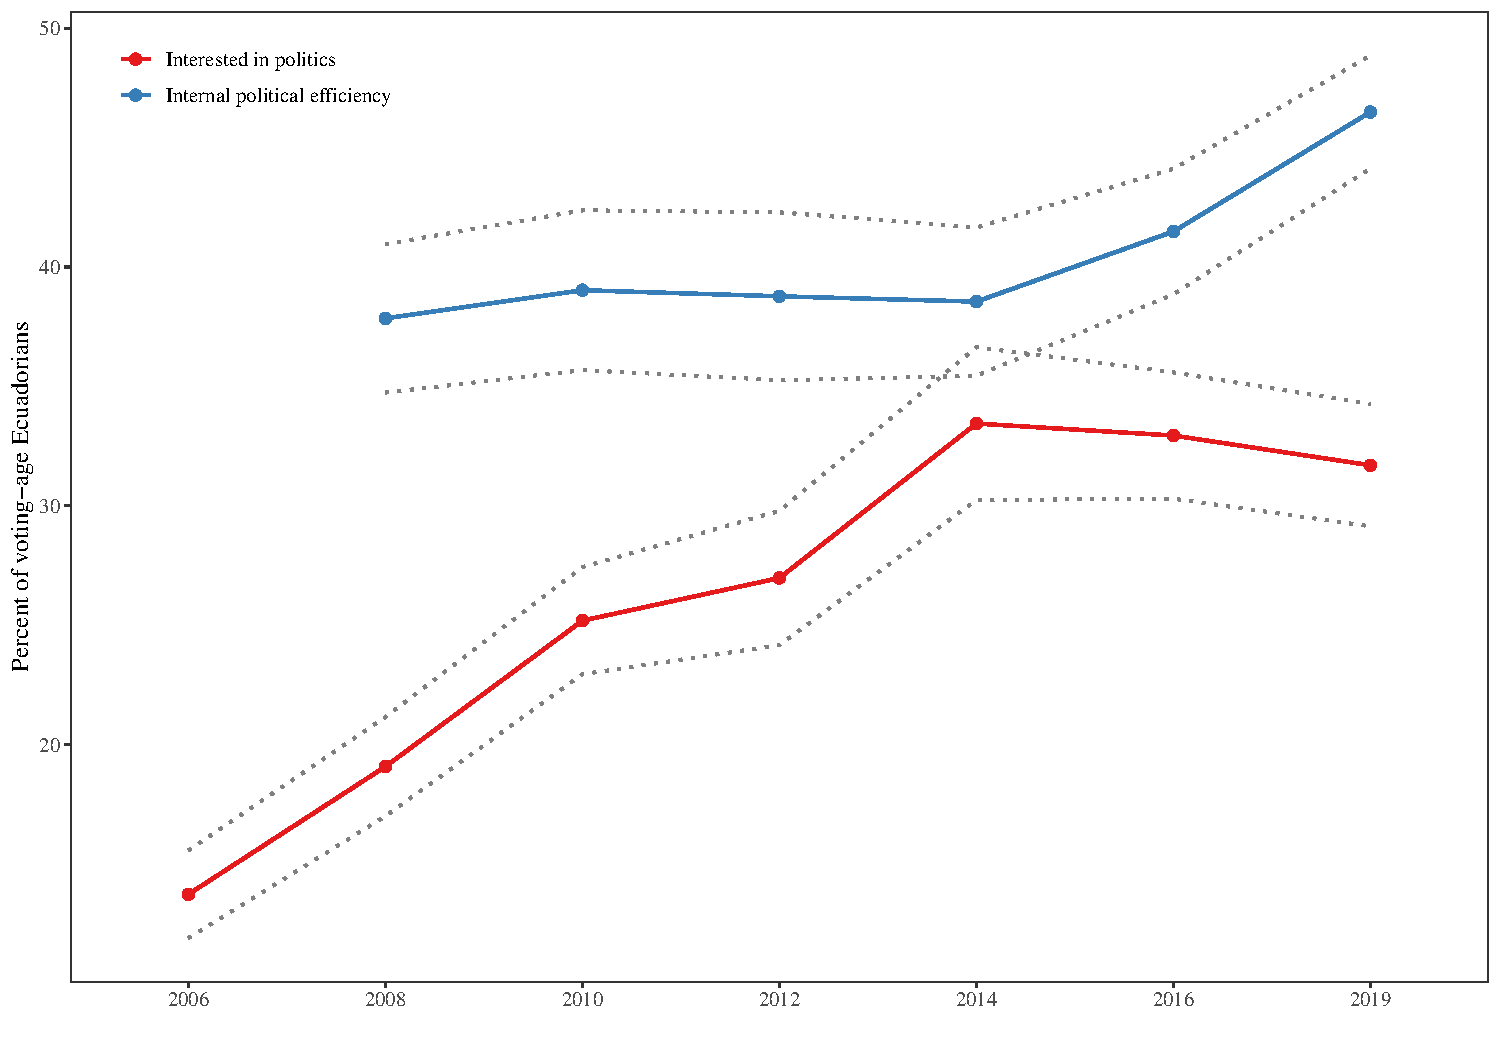
\includegraphics[width=\maxwidth]{figure/pol-int-graph-1} 

}


\end{knitrout}
\textbf{Note:} A time series of the internal political efficacy variable and the interest in politics variable. The internal political efficiency variable is dichotomized using the standard AB methodology as explained in \hyperref[app:first]{Appendix A}. Dotted lines represent the 95\% confidence intervals considering design effects. Data from the open-access AB databases. Figure prepared by the author.
\end{minipage}
}
\end{figure}
Figure \ref{fig:intpol} shows the percent who are interested in politics and also the percent who understand the country's politics. The gap between these two variables has increased from 2014 from 2016, and have a total historic correlation of 0.19. While they may appear to ask similar things, the two questions may imply different attitudes to politics: the political efficacy question simply asks if citizens are aware of politics and the second one asks if they're interested to enter the political scenario. It might be possible that, when separating these two questions, attitudes of apathy or pragmatism to the political society (understanding politics) are separated from an \enquote{idealist} attitude towards it of those who would like to enter politics.

A control for years of education is also added and it is significant, communicating that more educated respondents are less likely to justify corruption. Other things equal, an additional year of education is related to a 6 percentage points reduction in corruption tolerance. This finding is intuitive considering that more education may mean more knowledge about the costs of corruption. The social payoffs for being honest may be higher as also higher education may entail a better economic position which makes engaging in corrupt acts less economically attractive. 

Regarding the variables which measure corruption, it is possible to confirm findings by \textcite{Moscoso.2020}, \textcite{Lupu.2017} and \textcite{Singer.2016}: exposure to corrupt acts (paying or being asked to pay a bribe) is also strongly correlated with tolerance to them. A person who has been exposed to some form of bribing is about 15\% more likely to justify corruption according to the average partial effects in Table \ref{tab:apescomp}. The direction of causality is not clear in this case as it might be possible that a predisposed tolerance to corruption due to external factors makes citizens more likely to be in environments where corruption flourishes. \textcite{Moscoso.2018} finds that younger people and people with a higher number of children are more likely to be exposed to corruption with the 2016 Ecuador AB data. This may suggest that younger people justify corruption partly because they are more exposed by it: empirical models not shown explicitly show that an interaction term between age and corruption exposure is significant at the the 90\% confidence level. Corruption perceptions, on the other hand, play no role in determining corruption tolerance for this time period. This is also found by \textcite{Moscoso.2020} in 2019, however, \textcite{Lupu.2017} does find an effect of corruption perceptions on corruption tolerance for the whole Latin American region. An interaction term between year and corruption perceptions is not significant, although Figure \ref{fig:corrper} shows a significant increase of corruption perceptions between 2014 and 2016 (see \hyperref[app:first]{Appendix A}). 

% Make the corruption perceptions figure
\begin{figure}[htbp]
\fbox{
\begin{minipage}{\textwidth}
\caption{Corruption perceptions in Ecuador 2004-2016}
\label{fig:corrper}
\begin{knitrout}
\definecolor{shadecolor}{rgb}{0.969, 0.969, 0.969}\color{fgcolor}
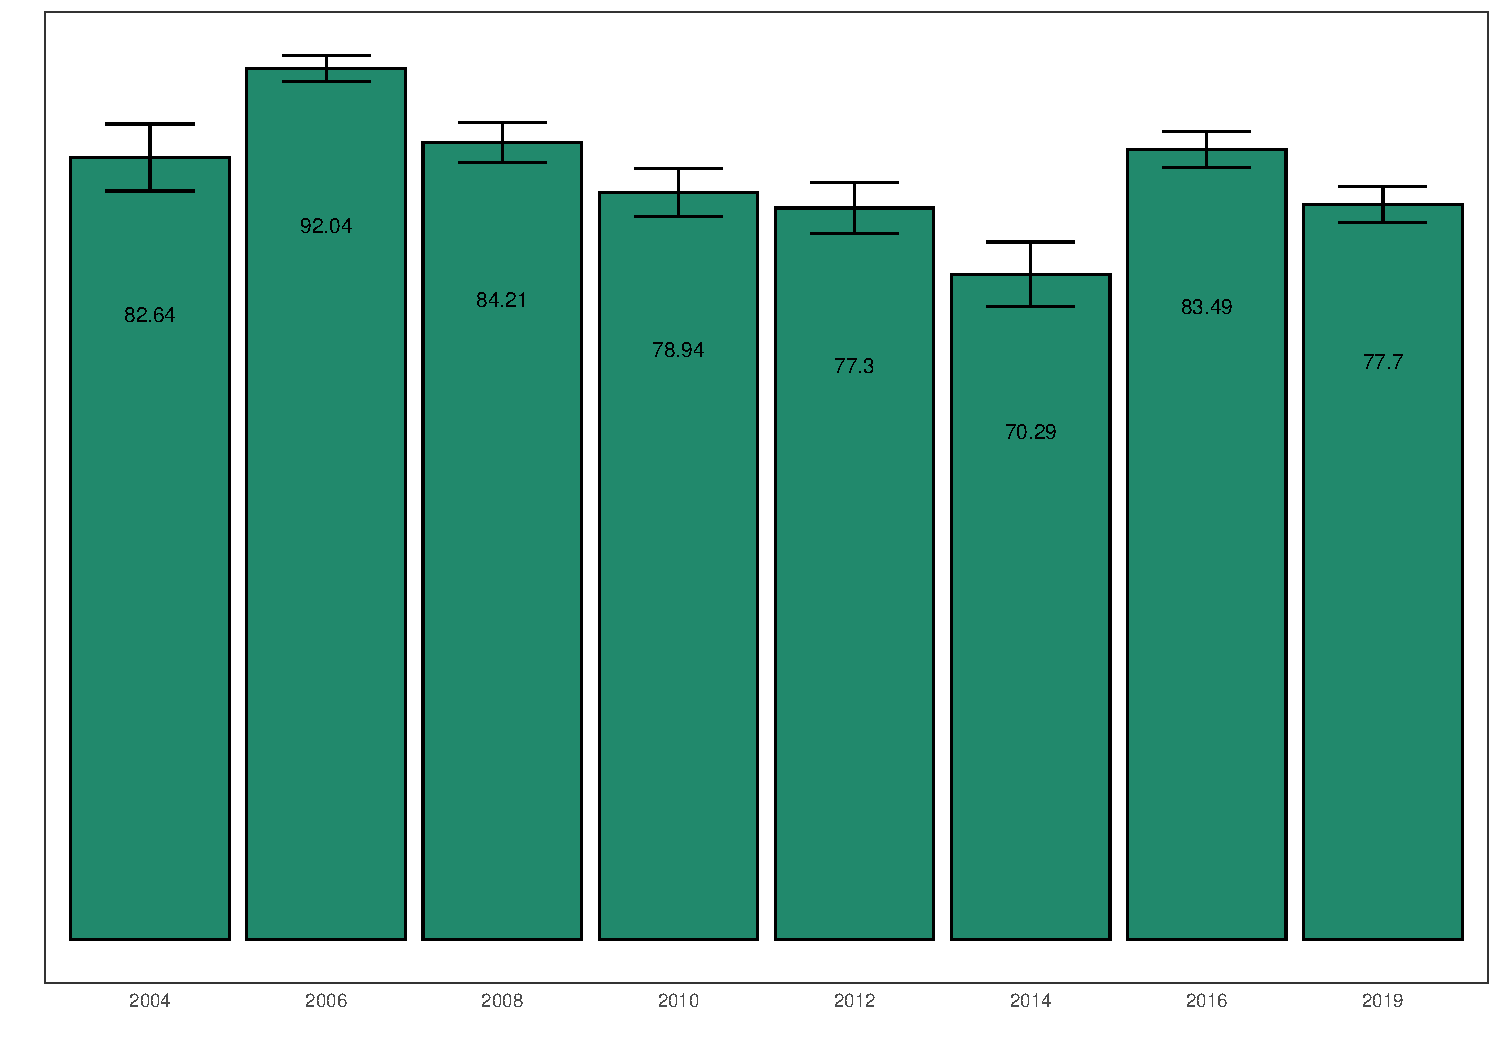
\includegraphics[width=\maxwidth]{figure/corrper_g-1} 
\end{knitrout}
\textbf{Note:} A time series of corruption perceptions in Ecuador. The corruption perceptions question was asked in a slightly different manner in 2016, thus the variable is recoded as explained in \hyperref[app:first]{Appendix A}, to construct this time series. Error bars represent the 95\% confidence intervals considering design effects. Data from the open-access AB databases. Figure prepared by the author.
\end{minipage}
}
\end{figure}

% Now the regressions which were not shown explicitly in text


A dummy variable equal to unity for respondents who have recently attended a protest is added and it is very significant. A person who has attended a protest is about 7\% more likely to justify corruption, other things equal. The reason why this happens might be related to a explanation of \textit{denial of victim} as proposed by \textcite{Ashforth.2003}. People who attend protests probably reject the current state of things, which may induce a feeling of contempt against society. They may believe dishonest acts could be justified in these adverse circumstances because they feel corrupt acts can be retribution to other dishonest acts done to them or by alleging that \textit{petty} corruption acts are nothing compared to grand corruption scandals. Since they have “declared” their rejection to the system in general, they have surrendered to its flaws and have no social incentives to remain honest.

Table \ref{tab:complexmod} also shows that after considering several variables suggested by the literature the interaction terms, as estimated in Table \ref{tab:simplemodel}, keep their sign and significance. Even after controlling for several important predictors of corruption tolerance, it is still true that unemployed people justified corruption more in 2014 but reduced their tolerance in 2016. People who approved the job performance of President Correa were less likely to justify corruption in both years, but their rejection of bribes was smaller in 2016. Finally, while the political identification was not important to predict corruption tolerance in 2014, it was significant in 2016; where people who identified as closer to the political right were more likely to justify corruption. To further explore the effects of these three key variables on corruption tolerance, cross-sectional models are estimated for 2014 and 2016 separately and shown below.



% Table of cross-sectional models
\begin{table}[htbp]
\begin{center}
\caption{Logit coefficients for cross-sectional models as seen in Equation \ref{eqn:crosssecmodel}}
\label{tab:crossmod}

\begin{tabular}[t]{lcc}
\toprule
  & (1) & (2)\\
\midrule
Constant & \num{-0.006} & \num{-0.110}\\
 & (\num{0.663}) & (\num{0.479})\\
Woman & \num{0.059} & \num{0.141}\\
 & (\num{0.204}) & (\num{0.133})\\
Age & \num{-0.019}*** & \num{-0.029}***\\
 & (\num{0.007}) & (\num{0.004})\\
Years of education & \num{-0.030} & \num{-0.047}***\\
 & (\num{0.030}) & (\num{0.018})\\
Lives in urban setting & \num{0.151} & \num{-0.075}\\
 & (\num{0.238}) & (\num{0.152})\\
External political efficacy & \num{-0.032} & \num{-0.056}\\
 & (\num{0.054}) & (\num{0.039})\\
Internal political efficacy & \num{0.164}* & \num{0.077}*\\
 & (\num{0.097}) & (\num{0.045})\\
Participation in a protest & \num{0.436} & \num{0.205}\\
 & (\num{0.301}) & (\num{0.275})\\
Interest in politics & \num{-0.265} & \num{-0.253}*\\
 & (\num{0.227}) & (\num{0.136})\\
Perceptions of corruption & \num{-0.005} & \num{0.112}\\
 & (\num{0.207}) & (\num{0.175})\\
Exposure to corruption & \num{1.520}*** & \num{0.663}***\\
 & (\num{0.178}) & (\num{0.145})\\
Unemployment & \num{0.942}*** & \num{0.042}\\
 & (\num{0.236}) & (\num{0.164})\\
Approval of Pres. performance & \num{-0.533}*** & \num{0.025}\\
 & (\num{0.108}) & (\num{0.072})\\
Political wing & \num{-0.025} & \num{0.053}**\\
 & (\num{0.040}) & (\num{0.022})\\
\midrule
$N$ & \num{1039} & \num{1269}\\
AIC & \num{755.79} & \num{1434.40}\\
BIC & \num{832.75} & \num{1516.11}\\
Year & 2014 & 2016\\
\bottomrule
\end{tabular}


\end{center}
\textbf{Note:} Logit models for the cross-sectional models for 2014 and 2016 as seen in Equation \ref{eqn:crosssecmodel}. Data from the open-access AB databases. Standard errors consider design effects of the AB complex survey design.\\
*$p$ < 0.1, **$p$< 0.05, ***$p$ < 0.01.
\end{table}

% Table of Cross-Sectional APEs
\begin{table}[htbp]
\begin{center}
\caption{Average partial effects for cross-sectional models in Table \ref{tab:crossmod}}
\label{tab:apecross}

\begin{tabular}[t]{lcc}
\toprule
  & (1) & (2)\\
\midrule
Age & \num{-0.002}*** & \num{-0.005}***\\
 & (\num{0.001}) & (\num{0.001})\\
Years of education & \num{-0.003} & \num{-0.009}***\\
 & (\num{0.003}) & (\num{0.003})\\
External political efficacy & \num{-0.003} & \num{-0.010}\\
 & (\num{0.006}) & (\num{0.007})\\
Internal political efficacy & \num{0.017}* & \num{0.014}*\\
 & (\num{0.010}) & (\num{0.008})\\
Interest in politics & \num{-0.028} & \num{-0.046}*\\
 & (\num{0.023}) & (\num{0.025})\\
Perceptions of corruption & \num{-0.001} & \num{0.021}\\
 & (\num{0.022}) & (\num{0.032})\\
Exposure to corruption & \num{0.192}*** & \num{0.132}***\\
 & (\num{0.026}) & (\num{0.030})\\
Unemployment & \num{0.122}*** & \num{0.008}\\
 & (\num{0.037}) & (\num{0.031})\\
Approval of Pres. performance & \num{-0.056}*** & \num{0.005}\\
 & (\num{0.012}) & (\num{0.013})\\
Political wing & \num{-0.003} & \num{0.010}**\\
 & (\num{0.004}) & (\num{0.004})\\
\midrule
$N$ & \num{1039} & \num{1269}\\
Year & 2014 & 2016\\
\bottomrule
\end{tabular}


\end{center}
\textbf{Note:} Average partial effects for logit cross-sectional empirical models in Table \ref{tab:crossmod}. Data from the open-access AB databases. Standard errors consider design effects of the AB complex survey design.\\
*$p$ < 0.1, **$p$< 0.05, ***$p$ < 0.01.
\end{table}

The coefficients shown in Table \ref{tab:crossmod} show that, while education is significant for the pooled regression, it is not for a 2014 cross-section: only in 2016 it is possible to detect a negative effect of education years in corruption tolerance. Table \ref{tab:apecross} shows that an additional year of education reduces the probability of justifying corruption by about 9 percentage points, all other things equal. A similar phenomenon is seen for the interest in politics variable: only in 2016 people who are interested in politics justify corruption more than those not interested. The exposure to corruption, internal political efficacy and age variables remain significant for both years. The effect of protest participation, while significant in the pooled regressions, is not significant in any of the individual years. 

The last rows of Table \ref{tab:crossmod} show the effects of the key regressors for 2014 ($\beta_{x^*}$ as defined in Equation \ref{eqn:crosssecmodel}). Model 1 shows that those who were unemployed justified corruption to a greater extent. However, as the interaction term in Table \ref{tab:crossmod} shows, the effect on unemployment for 2016 is smaller. The effect of unemployment or of any of the key regressors in 2016 can be understood as the \enquote{net} effect of the regressor as defined in Equation \ref{eqn:genmod}: $\beta_{x^*} + \delta_1 y_{16}$. In fact, according to the models in 2016 unemployed respondents do not display a different likelihood of justifying corruption relative to those who are not unemployed. The data shows that following the recession and loss of popularity of the regime, the unemployed remained approximately equal in their corruption tolerance proclivities relative to those who were not unemployed.

It is possible that initially unemployed people justified corruption more because it was their “steady state” of corruption tolerance: unemployed people are economically disadvantaged which gives them incentives to engage in corrupt actions which yield positive economic payoffs. Additionally, as they are unable to enter the job market for some time, they might feel more alienated from society, which might decrease social or moral incentives to remain honest by renouncing the economic payoffs that corruption may offer, as it has been explained previously. The change in corruption tolerance behavior for 2016 is more difficult to understand. It is possible that since the recession many lost their jobs and they have had relatively short unemployment spells. The recently unemployed may not feel too alienated from society and thus have not adopted an attitude of pragmatism toward the current circumstances. Savings or family income may support the recently unemployed which makes them feel less desperate and prone to take the “moral high ground”. This
all contributes to them still feeling part of society, which reduces their rationalization of corruption. However, with larger unemployment spells, desperation may trigger more pragmatic points of view, which will lead to higher corruption tolerance in future years. All of this contributes to the effect of unemployment in 2016 not being statistically different from zero, as seen in Table \ref{tab:crossmod}.

To better understand the implications of the political variables' coefficients and their change in time, consider a key actor on corruption normalization, leadership. Having initially branded himself as \enquote{the biblical underdog} \parencite[para. 4]{Hedgecoe.2009}, President Correa distanced himself from the country's political elite and constantly denounced  corruption and injustice in the system. The new government promised a radical change when it started its tenure in 2007 and did deliver as it gave Ecuador a politically stable though totalitarian environment, as well as other changes in political and economical mechanisms \parencite{Weisbrot.2017}. The President had explicitly stated that he would battle corruption and fiscal evasion \enquote{to the death} \parencite{Ortiz.2013}. Thus, supporters of this regime had higher social sanctions if they engaged in or justified corrupt behavior, as this may have implied that the economic and political model they supported was flawed.

However, by 2016 the popularity of the regime faced a sharp decrease. Several narratives started to be constructed by President Correa and his officials to explain the flaws and weaknesses that opponents had denounced. These included reducing corruption accusations to \enquote{political persecution} or unfounded claims done because of upcoming elections \parencite{Melendez.2017}. A statement by the President represents a particularly relevant example: a regime-affiliated newspaper portrayed how Correa qualifies the Panama Papers as a \textit{selective fight against corruption} which is nothing but another kind of corruption, as well as a \textit{strategy by power groups} to destabilize democratically-elect governments \parencite[para. 5-7]{Telegrafo.2016}. 

Even as corruption accusations had planted the seed of a deep investigation about a complex corruption scheme involving top government officials and large corporations \parencite{Villavicencio.2019}, authorities within the Correa administration reduced the importance of these events, which created a narrative for regime supporters. If the legitimacy of those who denounce and control corruption is questioned by an important authority of the organization, corrupt acts can be more easily normalized \parencite{Ashforth.2003}. Thus, if there was a greater incidence of corrupt acts as well as numerous attempts by the authorities to justify them, it can be understood how supporters of the regime started to justify corruption more.

The data also show how people who identify with the political right became more corruption-tolerant in 2016. It is not clear if there is a causal relationship involving the political right and corruption tolerance. This is because it has been determined that in Ecuador the answer to the political identification question has little to do with the traditional principles of the political wings that are commonly understood. Rather, it is possible that the political self-identification of Ecuadorians follows a multidimensional perspective \parencite{Moncagatta.2020b}, not too accurately measured with an indicator like the one used here. 

A potential explanation to the sign on this variable is that those who identify with the right do so partially because they consider themselves to be against the government in place. This is reasonable considering the increase in the percentage of "rightists" between 2014 and 2016, which moves together with regime's downfall. Additionally, it is possible that anti-regime attitudes formed under a common set of ideas rather than under a political party or figure, since during President Correa's tenure opposition forces did not materialize strongly behind a party or leader \parencite{Melendez.2017}. It is sensible to believe that no political wing has any particular preference for justifying or rejecting corruption, as important actors in both political wings have spoken against it, academics \parencite{Holcombe.2015} and politicians \parencite{Morris.2021} alike. However, anti-regime respondents rather than \enquote{rightists} might rationalize corruption as a form of revenge, as proposed by \textcite{Ashforth.2003} and noted by \textcite{Adoum.2000}.





\end{document}
